\section{Additional experiments}

\subsection{Visualizing breakdown of Assumption~\labelcref{item:lindeberg-condition}}

\cref{fig:time} demonstrates that our analytical model holds for long enough during training to capture the emergence of localization in the single ReLU neuron (\labelcref{item:single-neuron-model}). 
In the first three columns, we visualize the IPR of the weights from our empirical and analytical models, as well as the $\ell_2$ difference between these two weights.
In the first four rows, we visualize these metrics for four random initializations of the model, training each on $\texttt{NLGP}(g=100)$ with $\xi_0 = 0.3$ and $\xi_1 = 0.7$, where we expect from \cref{thm:localization} to see localization. 
We see the error rapidly increase shortly after IPR increases, indicating the formation of localized receptive fields.
The last three columns confirm this, as they show snapshots from \emph{before}, \emph{during}, and \emph{after} the divergence between the empirical and analytical weights.
We observe the weights are nearly identical \emph{before}, differ only slightly at the most localized point \emph{during}, and are both localized \emph{after}, but possibly with different magnitudes and positions.
The difference that emerges \emph{during} is due to a breakdown of Assumption~\labelcref{item:lindeberg-condition} used to create our analytical model, which is violated when the norm of $\mathbf{w}$ is dominated by just a few entries, \ie it is localized.
While \cite{ingrosso2022data} also observe a breakdown in their analytical model as localization emerges, ours, crucially, holds for long enough to characterize the emergence of localization.

We discuss the individual subplots in more detail.
In all but the third row of \cref{fig:time}, the analytical predictions are near-exact; in the third row, we predict localization, but at the wrong position.
Focusing again on the first row, we see that at $t=20$, the weights have not yet become localized (from IPR, left, first, and visually) and analytical and empirical weights match nearlt exactly, as confirmed by the small distance in left, center above. 
At $t=30$, a localized peak around $i=21$ begins to emerge, violating Assumption \labelcref{item:lindeberg-condition} and weakening analytical precision.
The analytical model then underestimates the degree to which the main peak at $i=21$ dominates, while it overestimates the size of competing peaks at $i=30$, $37$, and $90$. 
Despite this, at $t=50$, we see that predictions from the analytical model retain a match to the empirical model. 

In the last row of \cref{fig:time}, we use the same initialization and setting as in the first row, except that we train on $\texttt{NLGP}(g=0.01)$ data instead.
From \cref{thm:localization}, we \emph{do not} expect to see localization.
The evolution of IPR confirms this, as it stays low in magnitude.
We also see that, because localization never emerges, Assumption~\labelcref{item:lindeberg-condition} is never violated, and so our analytical model accounts for the empirical model nearly perfectly.

\begin{wrapfigure}{l}{0.45\textwidth}
    \centering
    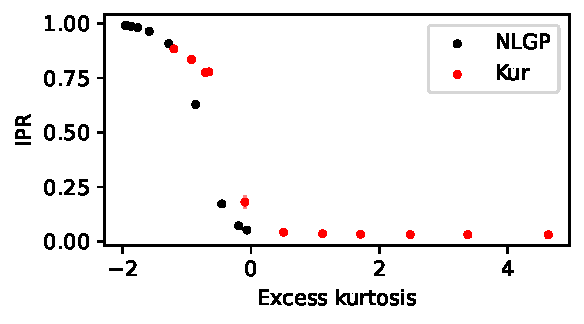
\includegraphics[width=170pt]{rebuttal-figures/replications/kurtosis_vs_ipr_40.pdf}
    \caption{
    IPR \vs excess kurtosis for $\texttt{NLGP}$ and $\texttt{Kur}$ data models, with mean and std.~dev.~across 30 re-initializations for the single-neuron model (\labelcref{item:single-neuron-model});
    error bars are small and may not be visible.
    }
    \label{fig:replications}
    \vspace{-14pt}
\end{wrapfigure}

